\documentclass[11pt]{article}

\usepackage[margin=0.85in]{geometry}
\usepackage{amsmath}
\usepackage{booktabs}
\usepackage{caption}
\usepackage{enumitem}
\usepackage{graphicx}
\usepackage{hyperref}
\usepackage{longtable}
\usepackage{tabularx}
\usepackage{xcolor}

\graphicspath{{figures/}}
\hypersetup{
  colorlinks=true,
  linkcolor=blue!50!black,
  urlcolor=blue!50!black
}
\captionsetup{font=small, labelfont=bf}
\setlist[itemize]{leftmargin=1.2em, itemsep=0.2em, topsep=0.3em}
\setlength{\parindent}{0pt}
\setlength{\parskip}{0.55em}

\newcommand{\policyFCFS}{pooled FCFS}
\newcommand{\policyStrict}{strict Class 1 reservation}
\newcommand{\servedrate}{\mathrm{served\_rate}}
\newcommand{\bookedrho}{\rho^{\mathrm{booked}}}
\newcommand{\attendedrho}{\rho^{\mathrm{attended}}}
\newcolumntype{Y}{>{\raggedright\arraybackslash}X}

\title{\vspace{-1.5em}Strict Class 1 Reservation vs FCFS\\
\large Utilization, Service-Rate, and Waiting-Time Tradeoffs}
\author{Short preliminary decision memo}
\date{}

\begin{document}
\maketitle

\section*{Executive Summary}

\textbf{Bottom line.} These results are preliminary and use only 5 seeds. Near the current baseline
($\lambda_1=\lambda_2=25$, total $\lambda=50$, $S=32$, $H=14$), strict reservation does
\textbf{not} beat pooled FCFS once the service-rate guardrail is checked. Both objective studies
select $Q=0$ at the baseline.

\begin{itemize}
  \item \textbf{Study A, utilization-first:} choose $Q$ by booked-slot utilization,
  $U_{\mathrm{util}}=\bookedrho$. At the baseline, the best choice is $Q=0$ and the strict-minus-FCFS
  difference is $+0.000$.
  \item \textbf{Study B, wait-adjusted:} choose $Q$ by booked-slot utility with Class 1 weight,
  a protected-slot penalty, and an offered-wait penalty. With $w_1=1.5$, $w_2=1.0$, $c=0.05$,
  and $\gamma=0.05$, the baseline best choice is also $Q=0$.
  \item \textbf{Guardrails matter.} Several high-$Q$ settings look better under the wait-adjusted
  utility, but they do so by shifting service strongly toward Class 1. Those settings fail the
  guardrail $\min_i \servedrate_i \ge 0.55$ and should not be treated as usable wins.
  \item \textbf{Interpretation.} Study A is the safer first-pass rule because it directly asks
  whether appointment capacity is booked. Study B is useful for understanding priority and wait
  tradeoffs, but only after service-rate constraints are enforced.
\end{itemize}

\section{Policy And Question}

The simulation compares two booking rules:

\begin{description}[leftmargin=1.8em, style=nextline]
  \item[Pooled FCFS] All patient classes compete for the same daily appointment capacity.
  \item[Strict Class 1 reservation] $Q$ slots per day are protected for Class 1. Class 1 can use
  protected slots first and then general slots. Class 2 can only use general slots. Unused protected
  slots remain empty.
\end{description}

The objective functions below are \textbf{after-the-fact scoring rules}. They do not change the
simulation policy. They are used to compare FCFS and strict reservation under matched scenarios and
matched seeds.

The main question is:

\begin{quote}
When, if ever, does strict Class 1 reservation outperform pooled FCFS, and what value of $Q$ is best
once utilization, service rates, waiting time, priority, and loss of pooling flexibility are included?
\end{quote}

\section{Notation And Baseline}

The notation follows the TeX reference files used by the simulation:

\begin{center}
\begin{tabularx}{0.92\linewidth}{@{}lX@{}}
\toprule
Symbol & Meaning \\
\midrule
$S$ & daily appointment capacity. In this run, $S=32$. \\
$H$ & rolling booking horizon. In this run, $H=14$. \\
$Q$ & protected Class 1 capacity per day. This is the policy parameter. \\
$\lambda_i$ & class-$i$ daily arrival rate. Baseline: $\lambda_1=\lambda_2=25$. \\
$\lambda$ & total daily arrival rate, $\lambda=\lambda_1+\lambda_2$. Baseline: $\lambda=50$. \\
$\tau$ & offered delay, in days. \\
$\bookedrho$ & booked-slot utilization: booked service-day slots divided by available measured slots. \\
$\attendedrho$ & attended utilization: completed visits divided by available measured slots. \\
$\servedrate_i$ & Class $i$ served rate: served Class $i$ arrivals divided by Class $i$ arrivals. \\
\bottomrule
\end{tabularx}
\end{center}

The demand sweep used here has equal arrivals for the two classes:
\[
  \lambda_1=\lambda_2 \in \{20,25,35,50\},
\]
so total demand is $\lambda \in \{40,50,70,100\}$. The seed set is 5101--5105.

\section{Objective Functions}

\subsection{Study A: Utilization-First With Service-Rate Guardrails}

The main score is booked-slot utilization:
\[
  U_{\mathrm{util}}(Q)=\bookedrho
  =\frac{\text{booked service-day slots}}{\text{available measured slots}}.
\]

Booked-slot utilization is used because it captures whether appointment capacity was scheduled,
including slots that later became no-shows. Attended utilization remains a diagnostic because it
measures completed visits.

The service-rate guardrail is:
\[
  \min\{\servedrate_1,\servedrate_2\} \ge 0.55,
  \qquad
  \servedrate_i=\frac{\text{served}_i}{\text{arrivals}_i}.
\]

The guardrail is not added to the objective. It decides whether a chosen $Q$ is acceptable.

\subsection{Study B: Wait-Adjusted Utility With Service-Rate Guardrails}

The weighted booked-slot term is:
\[
  U_{\mathrm{weighted\_booked}}(w_1,w_2)
  = w_1\bookedrho_1+w_2\bookedrho_2.
\]

The weighted offered delay is:
\[
  \bar{\tau}_w
  =
  \frac{
    w_1\sum \tau_{\mathrm{offered},1}
    +w_2\sum \tau_{\mathrm{offered},2}
  }{
    w_1\,\mathrm{offered}_1+w_2\,\mathrm{offered}_2
  }.
\]

The wait-adjusted objective is:
\[
  U_{\mathrm{wait\_util}}(Q)
  =
  U_{\mathrm{weighted\_booked}}(w_1,w_2)
  - c\frac{Q}{S}
  - \gamma\frac{\bar{\tau}_w}{H}.
\]

For the headline comparison:
\[
  w_1=1.5,\qquad w_2=1.0,\qquad c=0.05,\qquad \gamma=0.05,
  \qquad \min_i \servedrate_i \ge 0.55.
\]

The terms have simple roles: booked capacity is rewarded, Class 1 can be weighted more heavily,
protected capacity is penalized, and longer offered waits are penalized after normalizing by the
booking horizon.

\section{Main Results}

\subsection{Baseline Comparison}

At the baseline, both objective studies select $Q=0$. The smallest positive strict-reservation value
shown here, $Q=4$, has almost identical booked and attended utilization but a lower Study B score
after the protected-slot penalty.

\begin{center}
\small
\begin{tabularx}{\linewidth}{@{}Xrrrrrrrrrc@{}}
\toprule
Policy & $Q$ & $\bookedrho$ & $\attendedrho$ & SR$_1$ & SR$_2$ & Min SR & Wait & Study A & Study B & Feasible \\
\midrule
Pooled FCFS & 0 & 1.000 & 0.912 & 0.586 & 0.583 & 0.582 & 5.419 & 1.000 & 1.233 & yes \\
Selected $Q=0$ & 0 & 1.000 & 0.912 & 0.586 & 0.583 & 0.582 & 5.419 & 1.000 & 1.233 & yes \\
Strict, smallest positive $Q$ & 4 & 1.000 & 0.912 & 0.587 & 0.582 & 0.582 & 5.419 & 1.000 & 1.227 & yes \\
\bottomrule
\end{tabularx}
\end{center}

\begin{figure}[htbp]
  \centering
  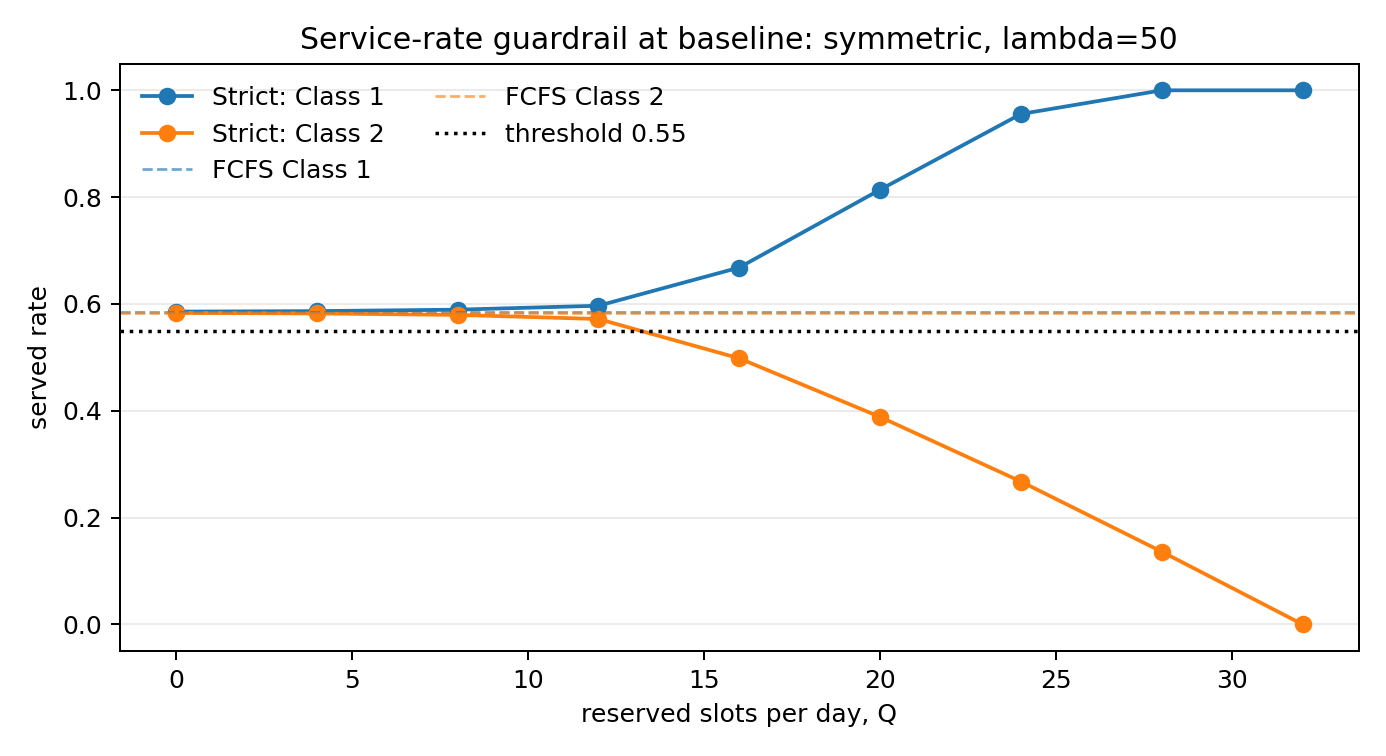
\includegraphics[width=0.86\linewidth]{service_rate_diagnostic_baseline.png}
  \caption{Baseline service-rate diagnostic. Dashed lines are FCFS references. The dotted line is the headline service-rate threshold, 0.55.}
\end{figure}

\subsection{Best \texorpdfstring{$Q$}{Q} By Scenario}

The two studies agree in 4 of the 12 scenario rows. Where they disagree, Study B often selects a
larger $Q$ because it rewards Class 1 access and wait improvements. Those selections usually fail
the minimum class served-rate guardrail.

\begin{center}
\scriptsize
\begin{tabularx}{\linewidth}{@{}Xrrrrc@{}}
\toprule
Scenario & A: best $Q$ & A feasible & B: best $Q$ & B feasible & Agree \\
\midrule
Symmetric, $\lambda=40$ & 0 & yes & 0 & yes & yes \\
Symmetric, $\lambda=50$ & 0 & yes & 0 & yes & yes \\
Symmetric, $\lambda=70$ & 0 & no & 32 & no & no \\
Symmetric, $\lambda=100$ & 0 & no & 32 & no & no \\
Class 1 advantaged, $\lambda=40$ & 0 & yes & 0 & yes & yes \\
Class 1 advantaged, $\lambda=50$ & 0 & no & 24 & no & no \\
Class 1 advantaged, $\lambda=70$ & 0 & no & 32 & no & no \\
Class 1 advantaged, $\lambda=100$ & 0 & no & 32 & no & no \\
Class 1 disadvantaged, $\lambda=40$ & 0 & yes & 16 & yes & no \\
Class 1 disadvantaged, $\lambda=50$ & 16 & yes & 16 & yes & yes \\
Class 1 disadvantaged, $\lambda=70$ & 0 & no & 32 & no & no \\
Class 1 disadvantaged, $\lambda=100$ & 0 & no & 32 & no & no \\
\bottomrule
\end{tabularx}
\end{center}

\begin{figure}[htbp]
  \centering
  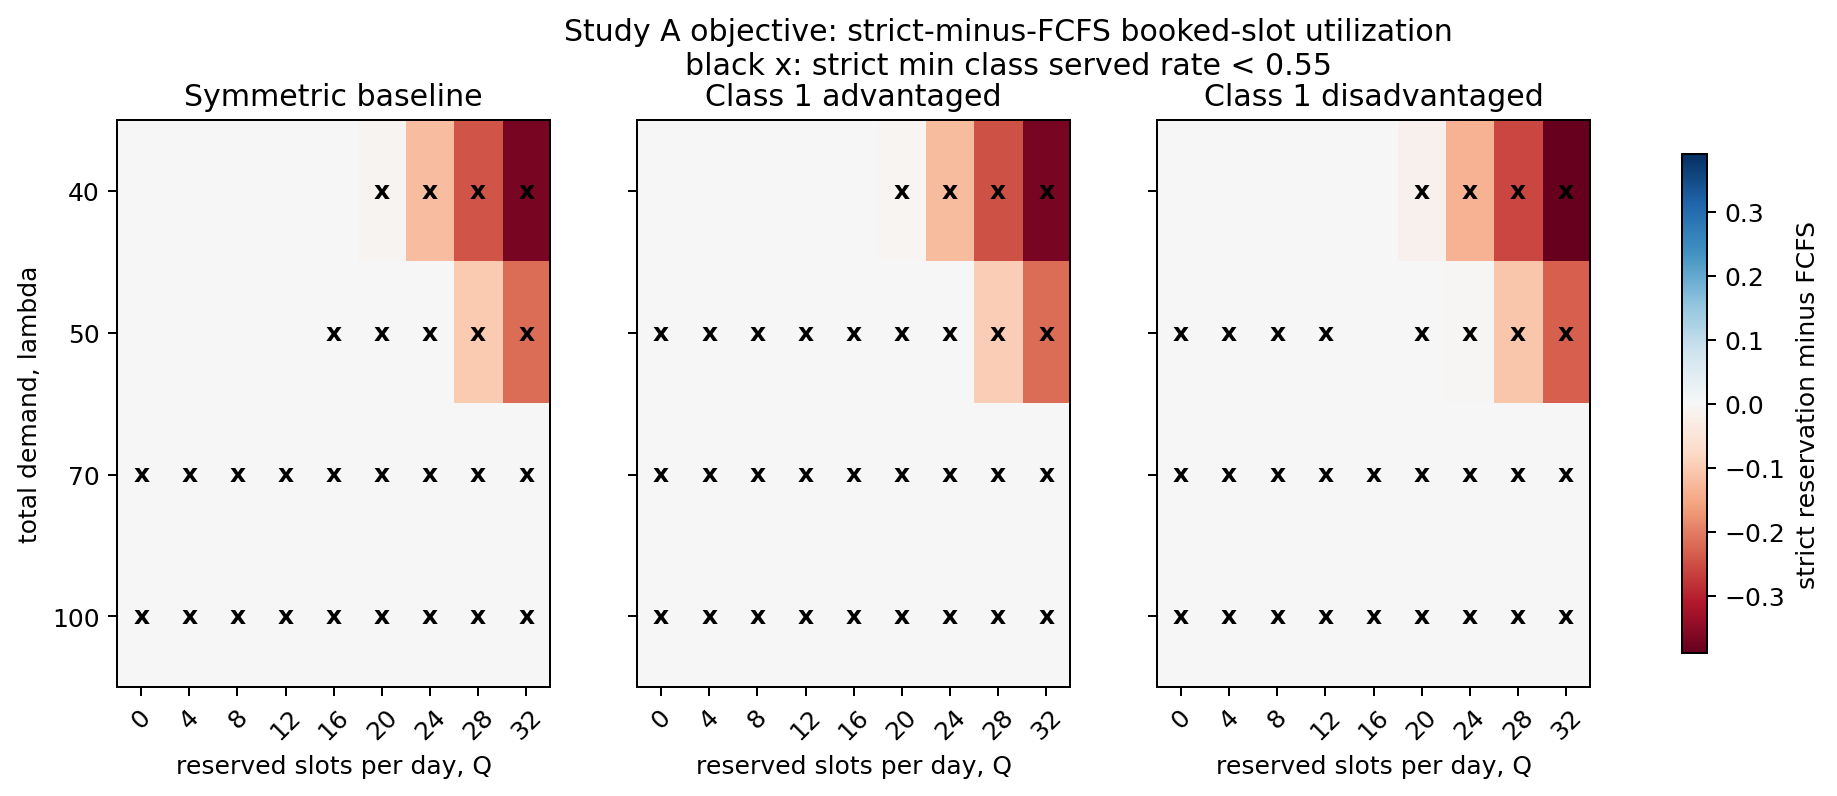
\includegraphics[width=\linewidth]{study_a_utilization_heatmap.png}
  \caption{Study A objective: strict-minus-FCFS booked-slot utilization. Black x marks cells where strict reservation violates the service-rate threshold.}
\end{figure}

\begin{figure}[htbp]
  \centering
  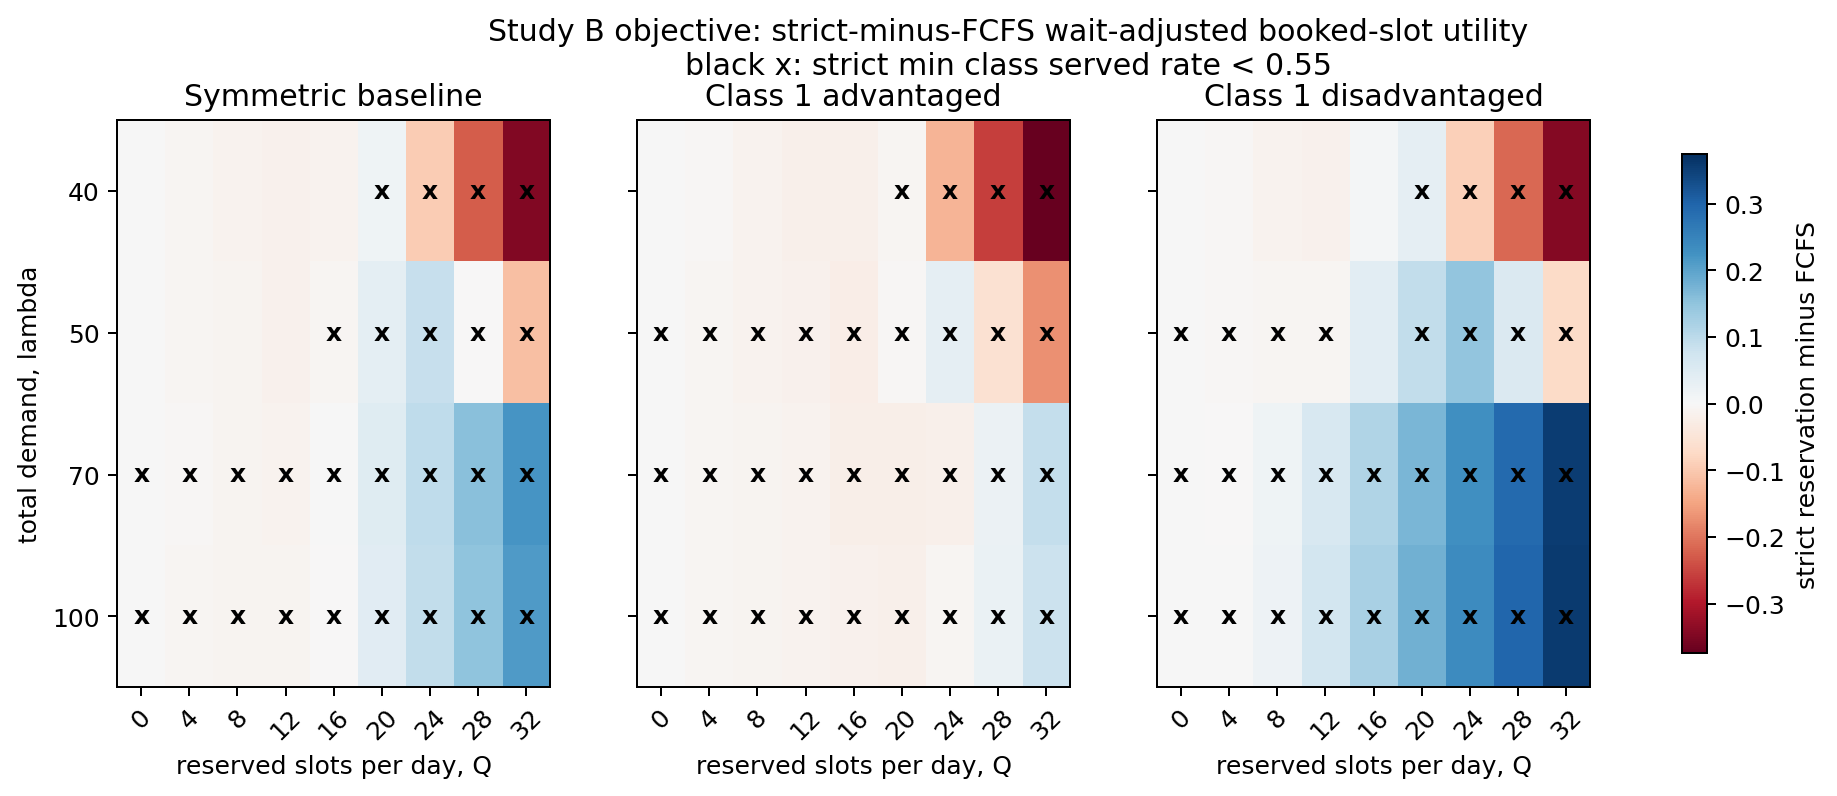
\includegraphics[width=\linewidth]{study_b_wait_adjusted_heatmap.png}
  \caption{Study B objective: strict-minus-FCFS wait-adjusted booked-slot utility. Black x marks cells where strict reservation violates the service-rate threshold.}
\end{figure}

\begin{figure}[htbp]
  \centering
  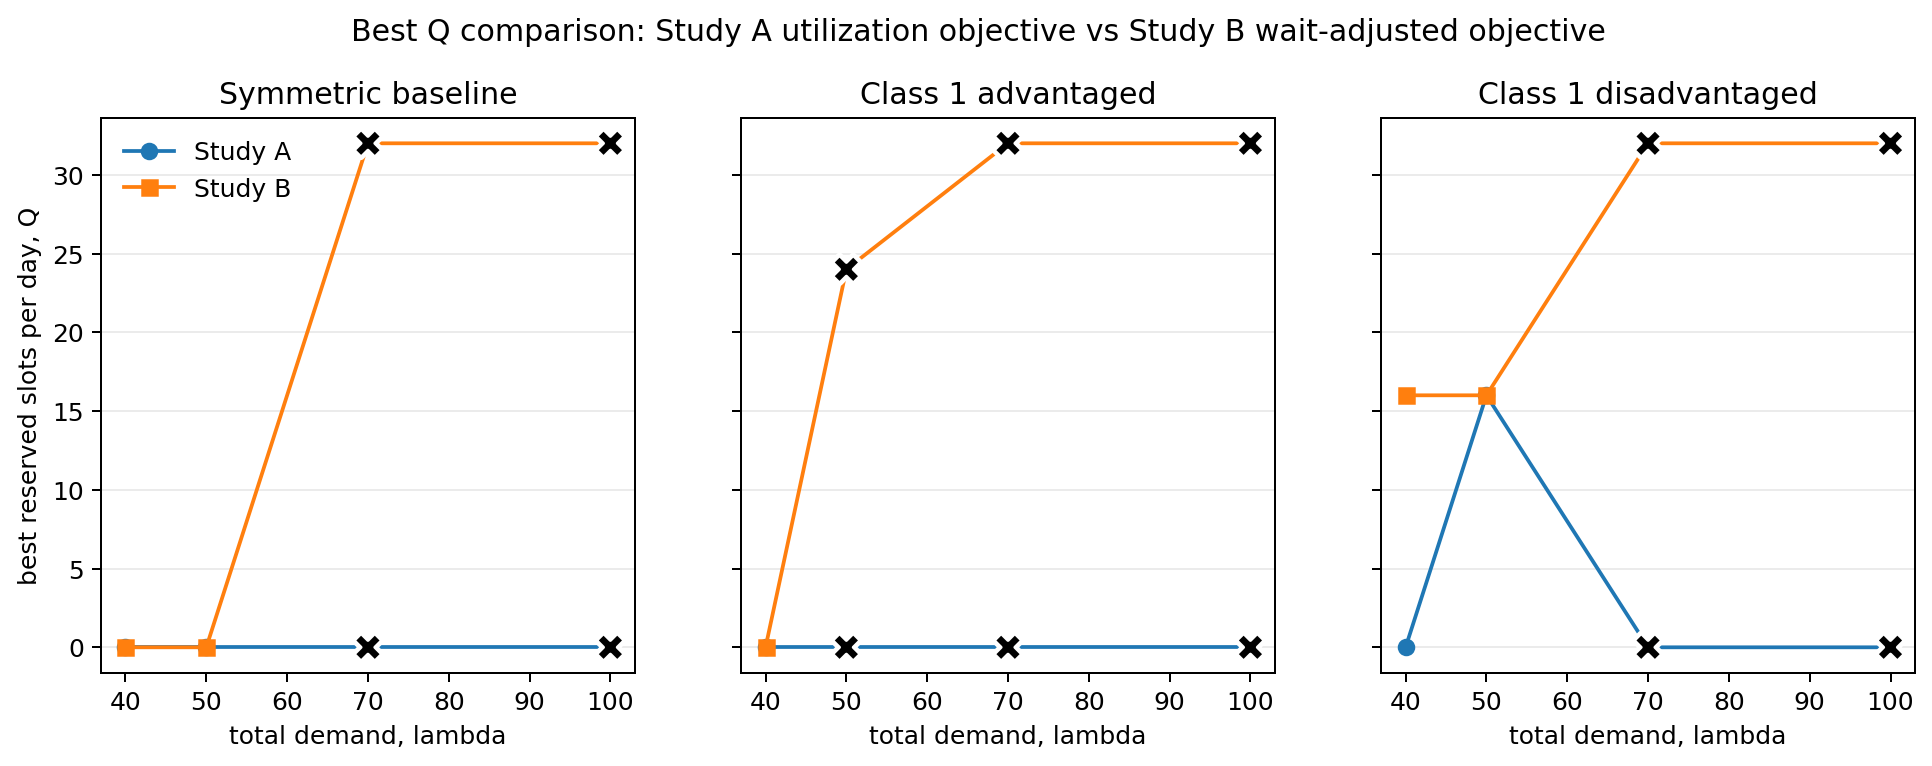
\includegraphics[width=\linewidth]{best_q_comparison.png}
  \caption{Best $Q$ under each study. Black X markers with a white outline mark infeasible selected values.}
\end{figure}

\begin{figure}[htbp]
  \centering
  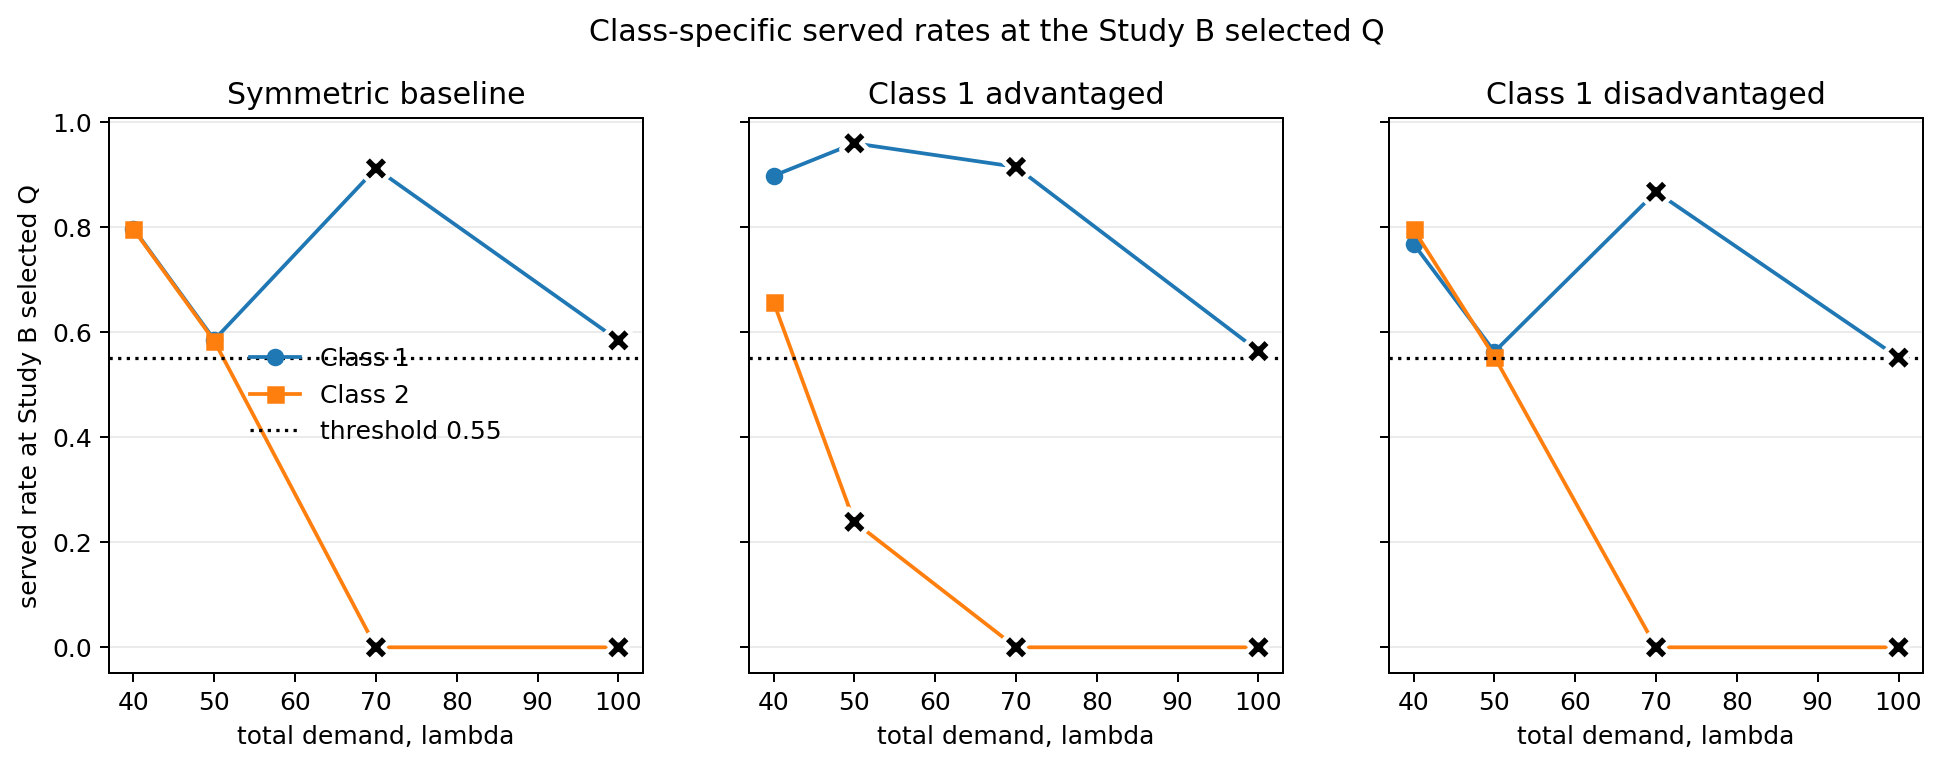
\includegraphics[width=\linewidth]{selected_q_class_served_rates.png}
  \caption{Class-specific served rates at the Study B selected $Q$. Class 1 and Class 2 are shown directly on the same axes; no class-advantage difference is plotted.}
\end{figure}

\section{Sensitivity}

The sensitivity table below focuses on the baseline setting and the headline Class 1 weight
$w_1=1.5$. The main pattern is clear: without a protected-slot cost ($c=0$), the wait-adjusted score
can select a positive $Q$. Once $c=0.05$ or $c=0.10$ is used, the selected baseline $Q$ returns to 0.

\begin{center}
\small
\begin{tabularx}{0.96\linewidth}{@{}lrrrrrcY@{}}
\toprule
Study & $w_1$ & $c$ & $\gamma$ & SR floor & Best $Q$ & Beats FCFS & Failure mode \\
\midrule
B & 1.5 & 0.00 & 0.00 & 0.55 & 12 & yes & none \\
B & 1.5 & 0.00 & 0.02 & 0.55 & 12 & yes & none \\
B & 1.5 & 0.00 & 0.05 & 0.55 & 12 & yes & none \\
B & 1.5 & 0.00 & 0.10 & 0.55 & 12 & yes & none \\
B & 1.5 & 0.05 & 0.00 & 0.55 & 0 & no & objective does not beat FCFS \\
B & 1.5 & 0.05 & 0.02 & 0.55 & 0 & no & objective does not beat FCFS \\
B & 1.5 & 0.05 & 0.05 & 0.55 & 0 & no & objective does not beat FCFS \\
B & 1.5 & 0.05 & 0.10 & 0.55 & 0 & no & objective does not beat FCFS \\
B & 1.5 & 0.10 & 0.00 & 0.55 & 0 & no & objective does not beat FCFS \\
B & 1.5 & 0.10 & 0.02 & 0.55 & 0 & no & objective does not beat FCFS \\
B & 1.5 & 0.10 & 0.05 & 0.55 & 0 & no & objective does not beat FCFS \\
B & 1.5 & 0.10 & 0.10 & 0.55 & 0 & no & objective does not beat FCFS \\
\bottomrule
\end{tabularx}
\end{center}

\begin{figure}[htbp]
  \centering
  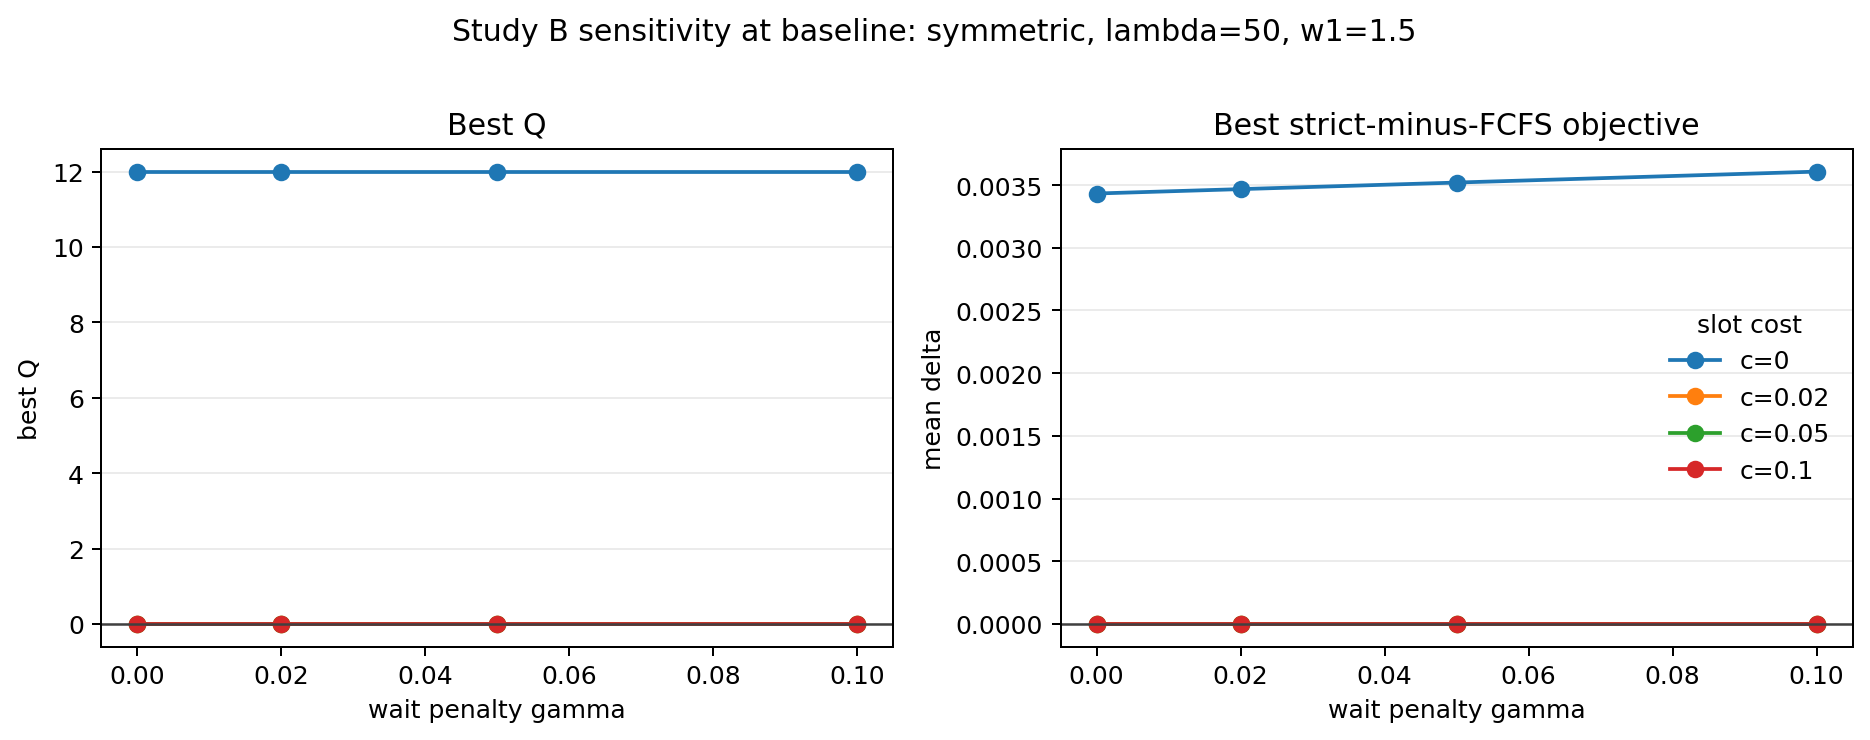
\includegraphics[width=0.88\linewidth]{gamma_sensitivity.png}
  \caption{Study B sensitivity at the baseline scenario. The plotted objective is the best strict-minus-FCFS wait-adjusted utility for each waiting-time penalty and slot-cost value.}
\end{figure}

\section{Decision Points Before Finalizing}

\begin{itemize}
  \item Confirm whether the service-rate floor should remain 0.55 or be raised.
  \item Decide whether booked-slot utilization is sufficient as the primary capacity target, or
  whether attended utilization should become a hard constraint because no-shows do not produce visits.
  \item Decide whether Class 2 served-rate loss should have its own explicit threshold.
  \item Rerun the sweep with more seeds before treating any $Q$ recommendation as final.
\end{itemize}

\section{Audit Notes}

\begin{itemize}
  \item Earlier objective-function wording from the draft has not been reused.
  \item This memo analyzes only the strict Class 1 reservation policy against pooled FCFS.
  \item The metric \texttt{booked\_slot\_utilization} is available in the simulation output.
  \item Class offered-delay totals and class service-rate guardrails are available.
  \item Each study uses one main objective for best-$Q$ selection.
\end{itemize}

\end{document}
